% This is "sig-alternate.tex" V2.1 April 2013
% This file should be compiled with V2.5 of "sig-alternate.cls" May 2012
%
% This example file demonstrates the use of the 'sig-alternate.cls'
% V2.5 LaTeX2e document class file. It is for those submitting
% articles to ACM Conference Proceedings WHO DO NOT WISH TO
% STRICTLY ADHERE TO THE SIGS (PUBS-BOARD-ENDORSED) STYLE.
% The 'sig-alternate.cls' file will produce a similar-looking,
% albeit, 'tighter' paper resulting in, invariably, fewer pages.
%
% ----------------------------------------------------------------------------------------------------------------
% This .tex file (and associated .cls V2.5) produces:
%       1) The Permission Statement
%       2) The Conference (location) Info information
%       3) The Copyright Line with ACM data
%       4) NO page numbers
%
% as against the acm_proc_article-sp.cls file which
% DOES NOT produce 1) thru' 3) above.
%
% Using 'sig-alternate.cls' you have control, however, from within
% the source .tex file, over both the CopyrightYear
% (defaulted to 200X) and the ACM Copyright Data
% (defaulted to X-XXXXX-XX-X/XX/XX).
% e.g.
% \CopyrightYear{2007} will cause 2007 to appear in the copyright line.
% \crdata{0-12345-67-8/90/12} will cause 0-12345-67-8/90/12 to appear in the copyright line.
%
% ---------------------------------------------------------------------------------------------------------------
% This .tex source is an example which *does* use
% the .bib file (from which the .bbl file % is produced).
% REMEMBER HOWEVER: After having produced the .bbl file,
% and prior to final submission, you *NEED* to 'insert'
% your .bbl file into your source .tex file so as to provide
% ONE 'self-contained' source file.
%
% ================= IF YOU HAVE QUESTIONS =======================
% Questions regarding the SIGS styles, SIGS policies and
% procedures, Conferences etc. should be sent to
% Adrienne Griscti (griscti@acm.org)
%
% Technical questions _only_ to
% Gerald Murray (murray@hq.acm.org)
% ===============================================================
%
% For tracking purposes - this is V2.0 - May 2012

\documentclass{sig-alternate-05-2015}

% Use Roman numerals for tables
\renewcommand{\thetable}{\Roman{table}}



\begin{document}

% Copyright
\setcopyright{acmcopyright}
%\setcopyright{acmlicensed}
%\setcopyright{rightsretained}
%\setcopyright{usgov}
%\setcopyright{usgovmixed}
%\setcopyright{cagov}
%\setcopyright{cagovmixed}


% DOI
% \doi{10.475/123_4}

% ISBN
% \isbn{123-4567-24-567/08/06}

%Conference
% \conferenceinfo{PLDI '13}{June 16--19, 2013, Seattle, WA, USA}

% \acmPrice{\$15.00}

%
% --- Author Metadata here ---
% \conferenceinfo{WOODSTOCK}{'97 El Paso, Texas USA}
%\CopyrightYear{2007} % Allows default copyright year (20XX) to be over-ridden - IF NEED BE.
%\crdata{0-12345-67-8/90/01}  % Allows default copyright data (0-89791-88-6/97/05) to be over-ridden - IF NEED BE.
% --- End of Author Metadata ---

\title{The Physical Benefits of VR games}
% \subtitle{[Extended Abstract]
% \titlenote{A full version of this paper is available as
% \textit{Author's Guide to Preparing ACM SIG Proceedings Using
% \LaTeX$2_\epsilon$\ and BibTeX} at
% \texttt{www.acm.org/eaddress.htm}}}
%
% You need the command \numberofauthors to handle the 'placement
% and alignment' of the authors beneath the title.
%
% For aesthetic reasons, we recommend 'three authors at a time'
% i.e. three 'name/affiliation blocks' be placed beneath the title.
%
% NOTE: You are NOT restricted in how many 'rows' of
% "name/affiliations" may appear. We just ask that you restrict
% the number of 'columns' to three.
%
% Because of the available 'opening page real-estate'
% we ask you to refrain from putting more than six authors
% (two rows with three columns) beneath the article title.
% More than six makes the first-page appear very cluttered indeed.
%
% Use the \alignauthor commands to handle the names
% and affiliations for an 'aesthetic maximum' of six authors.
% Add names, affiliations, addresses for
% the seventh etc. author(s) as the argument for the
% \additionalauthors command.
% These 'additional authors' will be output/set for you
% without further effort on your part as the last section in
% the body of your article BEFORE References or any Appendices.

\numberofauthors{8} %  in this sample file, there are a *total*
% of EIGHT authors. SIX appear on the 'first-page' (for formatting
% reasons) and the remaining two appear in the \additionalauthors section.
%
\author{
% You can go ahead and credit any number of authors here,
% e.g. one 'row of three' or two rows (consisting of one row of three
% and a second row of one, two or three).
%
% The command \alignauthor (no curly braces needed) should
% precede each author name, affiliation/snail-mail address and
% e-mail address. Additionally, tag each line of
% affiliation/address with \affaddr, and tag the
% e-mail address with \email.
%
% 1st. author
\alignauthor
Oona Kivelä \titlenote{Corresponding author}\\
    %    \email{trovato@corporation.com}
% 2nd. author
\alignauthor
Toni Kuosmanen 
% \email toni.kuosmanen@student.oulu.f
% 3rd. author
\alignauthor Timo Lämpsä
    %    \email{larst@affiliation.org}
\and  % use '\and' if you need 'another row' of author names
% 4th. author
\alignauthor Leevi Mustajärvi\\
% 5th. author
\alignauthor Joonas Soudunsaari\\
    %    \affaddr{NASA Ames Research Center}\\
    %    \affaddr{Moffett Field}\\
    %    \affaddr{California 94035}\\
    %    \email{fogartys@amesres.org}
}
% There's nothing stopping you putting the seventh, eighth, etc.
% author on the opening page (as the 'third row') but we ask,
% for aesthetic reasons that you place these 'additional authors'
% in the \additional authors block, viz.
\additionalauthors{Additional authors: John Smith (The Th{\o}rv{\"a}ld Group,
email: {\texttt{jsmith@affiliation.org}}) and Julius P.~Kumquat
(The Kumquat Consortium, email: {\texttt{jpkumquat@consortium.net}}).}
\date{30 July 1999}
% Just remember to make sure that the TOTAL number of authors
% is the number that will appear on the first page PLUS the
% number that will appear in the \additionalauthors section.

\maketitle
\begin{abstract}
% This paper provides a sample of a \LaTeX\ document which conforms,
% somewhat loosely, to the formatting guidelines for
% ACM SIG Proceedings. It is an {\em alternate} style which produces
% a {\em tighter-looking} paper and was designed in response to
% concerns expressed, by authors, over page-budgets.
% It complements the document \textit{Author's (Alternate) Guide to
% Preparing ACM SIG Proceedings Using \LaTeX$2_\epsilon$\ and Bib\TeX}.
% This source file has been written with the intention of being
% compiled under \LaTeX$2_\epsilon$\ and .

% The developers have tried to include every imaginable sort
% of ``bells and whistles", such as a subtitle, footnotes on
% title, subtitle and authors, as well as in the text, and
% every optional component (e.g. Acknowledgments, Additional
% Authors, Appendices), not to mention examples of
% equations, theorems, tables and figures.

% To make best use of this sample document, run it through \LaTeX\
% and BibTeX, and compare this source code with the printed
% output produced by the dvi file. A compiled PDF version
% is available on the web page to help you with the
% `look and feel'.
\end{abstract}


%
% The code below should be generated by the tool at
% http://dl.acm.org/ccs.cfm
% Please copy and paste the code instead of the example below. 
%
% \begin{CCSXML}
% <ccs2012>
%  <concept>
%   <concept_id>10010520.10010553.10010562</concept_id>
%   <concept_desc>Computer systems organization~Embedded systems</concept_desc>
%   <concept_significance>500</concept_significance>
%  </concept>
%  <concept>
%   <concept_id>10010520.10010575.10010755</concept_id>
%   <concept_desc>Computer systems organization~Redundancy</concept_desc>
%   <concept_significance>300</concept_significance>
%  </concept>
%  <concept>
%   <concept_id>10010520.10010553.10010554</concept_id>
%   <concept_desc>Computer systems organization~Robotics</concept_desc>
%   <concept_significance>100</concept_significance>
%  </concept>
%  <concept>
%   <concept_id>10003033.10003083.10003095</concept_id>
%   <concept_desc>Networks~Network reliability</concept_desc>
%   <concept_significance>100</concept_significance>
%  </concept>
% </ccs2012>  
% \end{CCSXML}

% \ccsdesc[500]{Computer systems organization~Embedded systems}
% \ccsdesc[300]{Computer systems organization~Redundancy}
% \ccsdesc{Computer systems organization~Robotics}
% \ccsdesc[100]{Networks~Network reliability}


%
% End generated code
%

%
%  Use this command to print the description
%
\printccsdesc

% We no longer use \terms command
%\terms{Theory}

\keywords{ACM proceedings; \LaTeX; text tagging}

\section{INTRODUCTION AND MOTIVATION}
The aim of this study is to detect the physical benefits in virtual reality 
(VR) gaming. To get to the goal the heart rate of the subjects is going to 
be measured in rest and during the game. Also, subjects are asked to fill 
questionnaire about their exercise and gaming habits. There is also going 
to be question about the VR game experience. The goal is to see if VR games 
have physical effects in user and also if user enjoys exercising with the 
VR game.

While deciding the research area we get motivated by the paper of Finkelstein 
et al. (2011). Their study was about motivation to exercise by exergames. 
They designed game called Astrojumper which forces the user to move his/her 
whole body while playing. Player flies in outer space and swerve around, 
duck under and jump over virtual planets. They studied the effectiveness 
of this kind of game by measuring the heart rate before the game session 
and after the game session. One game session lasted 15 minutes. To get 
more information about the motivational part of the game they also asked 
the test users to fill pre- and post-questionnaires. Pre-questionnaire 
included more general information about users exercise habits and experiment 
with video games. In post-questionnaire the questions were focused on to 
the game session. It was shown that virtual reality games have strong 
potential to motivate to physical activity both adults and children.

Finkelstein et al. (2011) made their research seven years ago and the VR 
equipment are highly improved since then. In their study a user had a 
control backpack in his/hers back with many wires leading from there. 
The game setting in Astrojumper is highly different than what we are using 
in our study. The monitors are placed around the user while we are going 
to use VR glasses. Movement trackers are on the forehead, wrists and waist 
in the Astrojumper. This also forced the user to move his/her whole body 
while we are having games only with controller sticks. In our study we 
are using VR glasses with wireless control sticks. In Finkelstein et al. 
(2011) study they had problems with heart rate measurements during the game 
session and we try to avoid those problems by using newer technique. 

\section{RELATED WORK}
\subsection{Virtual reality games}
If the system consists a human operator, a human-machine interface and 
a computer it can be called a virtual environment. Environment has 
three-dimensional space where the objects are placed. 
(Durlach \& Mavor 1995). Virtual reality games are characterized by high 
level of presence and immersion, or the feeling of really being a part 
of the virtual environment (Steuer, J. 1992).

Adaptation of VR systems has been partly hampered by many users 
experiencing a set of symptoms similar to motion sickness. This set 
of symptoms is commonly called cybersickness. Possible symptoms include 
but are not limited to nausea, dizziness, headaches and fatigue. 
Studies have estimated that 30 \% - 80 \% percent of VR users 
experience these symptoms to some extent (Rebenitsch \& Owen, 2016).

\subsubsection{HTC Vive, Oculus and Sony Playstation}
In recent years, many new consumer virtual reality systems have entered 
the market. Commonly these systems include an immersive head mounted 
display (HMD) and motion controllers. Popular examples of these systems 
include products such as Oculus Rift, HTC Vive or Playstation VR. Advanced 
head tracking and motion controllers combine to produce a high level of 
immersion and allow the user to explore and interact with their immediate 
surroundings in a natural fashion. Although Amazon sales rankings have 
recently shown a declining interest in VR devices (Fruhlinger, 2018), 
millions of devices have been shipped worldwide.

\subsubsection{Exergames}
Exergame term is widely used when video games are played to promote 
physical activity (Oh \& Yang, 2010). Children are easier to motivate 
to exercise with a fun way and childhood obesity can be prevent by 
exergames (Staiano et al. 2013). According to Staiano et al. (2013) 
children who were competitive exergames did not lose weight while 
cooperative “exergamers” did. Studies with elderly shows that with 
them the fun is not the driven force to play but the usefulness of 
the related physical and cognitive abilities is (Chen et al. 2018).

Study conducted by Plante et al. (2003) found evidence that combining 
VR with physical exercise can boost the mood benefits associated with 
normal exercise. In the study people who were immersed in a virtual 
environment while riding an exercise bike generally reported feeling 
more energized and less tired than the people in the control group 
(Plante et al. 2003). 

Fitzgerald et al. (2010) have shown that exergames has been used successfully 
also in therapy. They used a wobble-board based on video game to motivate 
the patients. Their results show that patients are more motivated for 
training when comparing to those who does similar exercises at a class 
with a therapist. Dynamic stability in both test groups gained and there 
were no significant differences between groups. (Fitzgerald et al. 2010)

\subsection{Heart rate and exercise intensity}
Heart rate measurements have long been used to monitor exercise intensity 
(Achten \& Jeukendrup 2003). A common way to represent exercise intensity 
using heart rate is to calculate the current heart rate as a percentage 
of the maximum heart rate: 

\begin{equation}\%HR = \frac{HR}{HR_{max}}\end{equation}

Although the maximum heart rate varies greatly between individuals, 
it can be estimated without measurement if the persons age is known. 
For example, Robergs et al. (2002) suggest the formula:

\begin{equation}HR_{max} = 205.8 - 0.685 * age\end{equation}

as the most acceptable estimate of maximum heart rate. Gulati et al. 
(2010) propose a slightly different age scaling factor of 0.88 for women. 
United States Center of Disease Control (2015) recommends target heart 
rates of 50 - 70 \% for moderate exercise and 70 - 85 \% for vigorous 
exercise.

\section{SENSING APPLICATION}
\subsection{Design}
Our research is based around VR games. VR game set includes VR glasses, 
motion controllers, base stations and a computer. The purpose is to track 
the movement, our goal is to capture the data directly from the VR 
hardware. 

Measuring the heart rate, we use sensor that allows continuous measurement 
during test. The best solution is to have a heart rate monitor which can 
be attached to player’s wrist since it will not fall or start moving so 
easily. Additionally, we measure the resting heart rate before performance.

Participants are going to be interviewed before game session, between two 
game sessions and after both game sessions. Participants are asked to 
answer questions about their general background, exercising background, 
gaming background and about the VR game experience. We also ask if user 
felt any cybersickness during or after the game sessions. 

There will be used two different games and each participant will play both. 
Other game is more hectic, an exergame-like game, and other is easier going.

\subsubsection{Cybersickness and heart rate}
As mentioned earlier, many VR users experience some degree of cybersickness. 
High levels of nausea can lead to increased heart rate without any physical 
activity (Nalivaiko et al. 2015). In order to find out if the observed increase 
in heart rate is caused by onset of cybersickness instead of exercise, we ask 
our test users the Simulator Sickness Questionnaire (SSQ) (Kennedy et al. 1993) 
after the game sessions. The SSQ, which was originally developed for military air 
simulation use, has been widely used in cybersickness research. The SSQ measures 
16 different symptoms on a four-point scale. The symptoms are grouped to three 
different categories: oculomotor symptoms, disorientation, and nausea. From 
the raw data a score for each of the three main symptom categories and a total 
score can be calculated (SSQ-O, SSQ-D, SSQ-N, and SSQ-T respectively). As nausea 
is the symptom mostly linked with increased heart rate, we will have to keep an 
eye on the SSQ-N scores.

\subsection{Implementation}
VR gaming device which includes HTC Vive visor, two motion controllers and 
two base stations are set in demo room inside Oulu university faculty of 
information technology and electrical engineering. We gather 17 participants 
to play two different games and we measure heart rate and movement data from 
them while they are playing. For heart rate measurement we are using two 
Fitbit Charge HR wristband devices as other one can be placed on next participant’s 
wrist while he/she is waiting his/her turn. Also, if either of the devices 
stops working, we can still use the other one for measuring. This way we 
can ensure data collection and keep the game sessions going on fluently. 
Data from these devices are synchronized to Fitbit web service via Fitbit 
mobile application. Heart rate data is extracted from these devices afterwards 
using 3rd party web service called “Pulse Watch” and exported to csv-file which 
can be then downloaded for further analyzing. Collected heart rate data will 
be from each second during game session.

For movement data collecting we are using additional capture software which 
is run parallel to the VR game. This software will collect position data from 
VR visor and two motion controllers and save that position data with timestamps 
to a plain text file for later analysis. 

At the beginning the participant is sat down and Fitbit heart rate bracelet 
is attached to their wrist. Then participants will be interviewed. Interview 
includes question about their background of exercising, video games and general. 
They are also asked to fill consent form (Attachment 1). Interview continues after 
first gaming session with questions about the exact gaming session. After second 
gaming session participants are interviewed with questions about the latter gaming 
session. Final interview also includes questions about SSQ, and questions based 
on their experience about exergames. 

We start each game session by introducing participant to the game he/she will be 
playing. Participant will be given 10 minutes of time to play each of the games. 
Each participant will be given an ID number which is then used to connect heart 
rate data, movement data and questionnaire answers together.

\section{EVALUATION}
\subsection{Evaluation plan}
Based on the study results, we are trying to find clear evidence that 
playing VR games really have health benefits and they activate and 
inspire people to move more than usually. We are also keen on finding 
results we did not expect based on interviews and data analysis.

We will compare heart rates of the user between two different VR games 
to detect if the exergame have raised users heart rate. We also detect 
the movements of hands and head during game session to compare if the 
exergame has moved users. By movement detection we exclude users heart 
rate increase caused by excitement. 

Interview results may also be interested here. Even we hope to detect 
that more hectic game, BeatSaber, moves people more and raises their 
heart beat than QuiVR, participants may still think that it is neither 
fun nor exercising. It is also interesting to see if people would more 
easily recommend exergames to others instead of using those by themselves. 
It would also be interesting to see whether users rate more hectic 
BeatSaber being more intense than QuiVR. It is interesting to see if the 
game order matters to users thoughts.

\subsection{Research data}
During the game session we gathered three types of data from test users. 
We gave them a Fitbit bracelet which measured heart rate in real time. 
We collected qualitative data from users by interviewing users before 
game session, after first game session and finally after second game 
session. We also had SSQ interview to participants. We gathered movement 
data from hand consoles and VR glasses via capture software which was 
run parallel to the VR game.
\subsubsection{Interview data}
Test users were at the beginning asked to fill consent form. 
There their permission to use their data in this study was asked. After 
users were given their permission, the interviews were continued. First, 
they were asked some general information about their age and gender. 
Age information was gathered in order to calculate theoretical maximum 
heart rate. Low rate of women participants prevents data comparison 
between genders. In the interview, users’ weekly activity with sports 
and with computer or console games were asked as for background information. 
Users were also asked if they have used VR applications before. After first 
phase interview user played ten minutes either BeatSaber or QuiVR game. 

After first game session interview was continued by asking how user was 
feeling after the game. Users’ were also asked how intense they would 
rate the game session in a scale from one to five. User then played 
ten minutes the second game.

After second game session user were asked again how they feel, and 
how intense they would rate the game session. To cut off the effect 
of simulator sickness, user was asked sixteen questions according 
to Kennedy et al. (1993) SSQ. Next part of the interview we asked 
if user sees himself/herself playing VR games for exercise meaning 
and for fun in scale one to five. And for final part we asked, 
would user play virtual reality games in exercise context and would 
he/she recommend that to others in scale one to five. Users had 
also a chance to say any comment about the whole experience.

Interview results about user’s physical activity and computer or 
console game activity, as well as if user would play VR games and 
if user would play them for exercise purpose or if they would 
encourage user to exercise more and if user would recommend VR 
games for exercise purpose to someone else, are shown in Table I. 
Users were also asked to rank the intense of the game session 
(from scale 1 to 5) after each session. Their results are shown 
in Figure 1. 

\begin{figure}
\centering
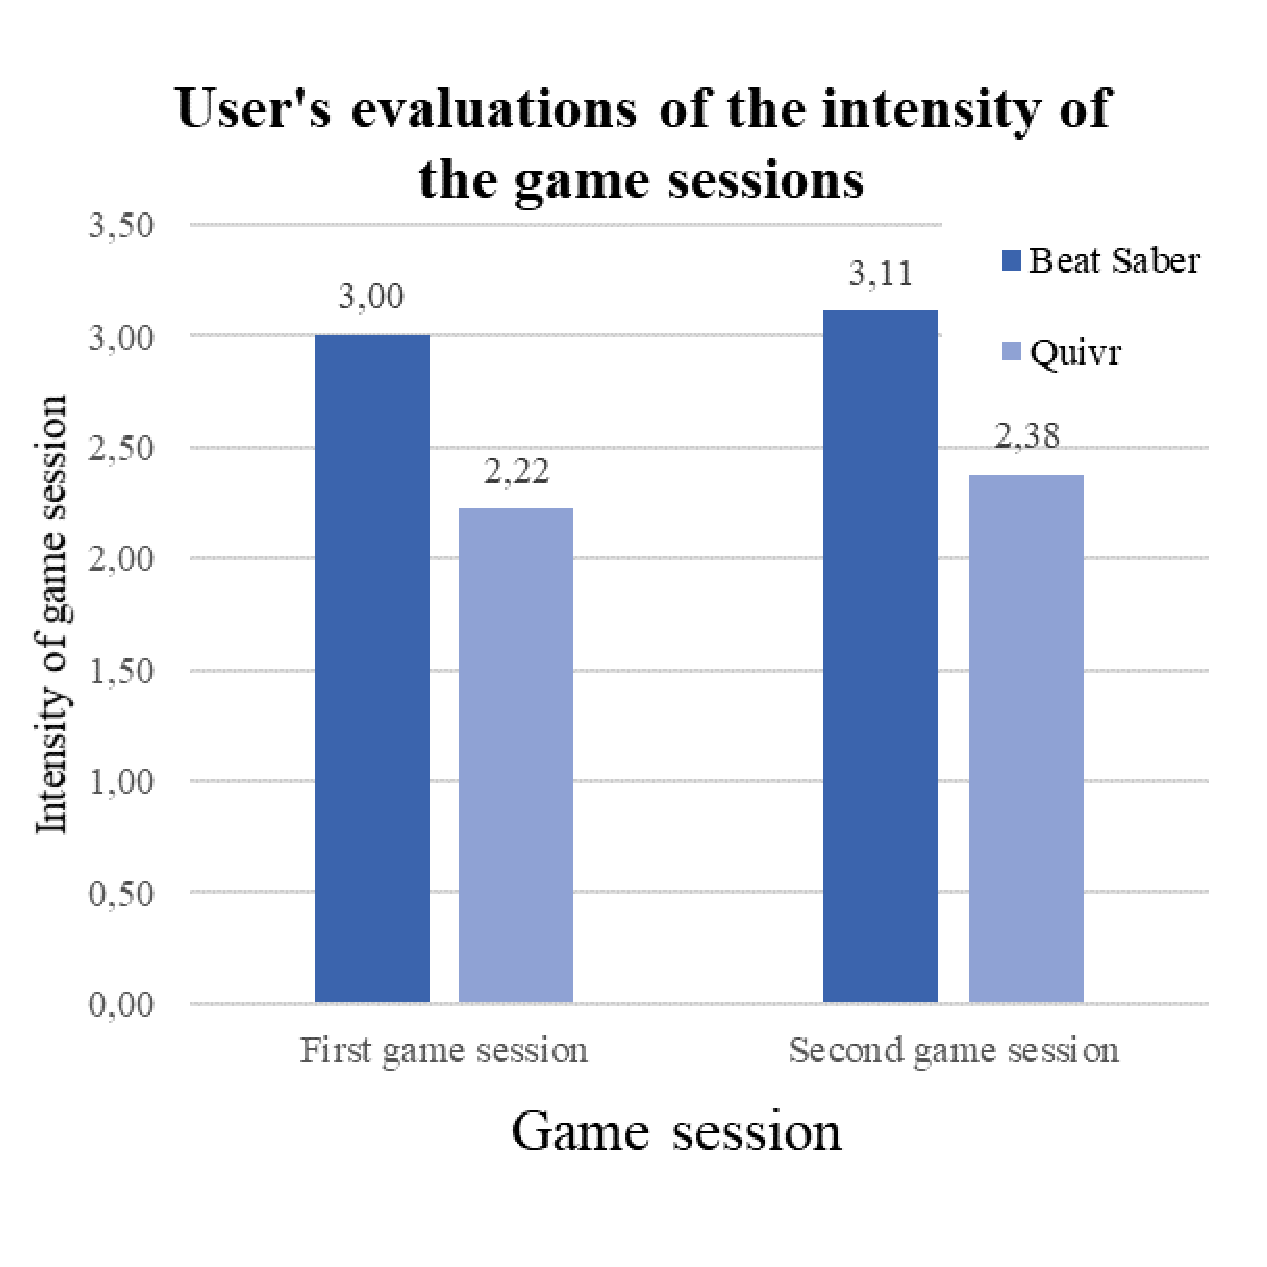
\includegraphics{intensity_evaluation}
\caption
    {
        Users evaluation of intense of game session. 
    }
\end{figure}

\begin{table*}
\centering
\caption
{
    Survey results.\newline
    Q1: How many times a week you do sports? (at least 30 mins of exercising per time)\newline
    Q2: How many hours do you usually play computer games or console games in a week?\newline
    Q3: Could you see yourself playing virtual reality games more often just for fun?\newline
    Q4: Could you see yourself playing a virtual reality games more often for exercise purposes?\newline
    Q5: Would VR playing encourage you to exercise more?\newline
    Q6: Would you recommend VR gaming as an exercise for anyone?\newline
}
\begin{tabular}{c|c c c c c c} \hline
    % ID&How many times a week you do sports? (at least 30 mins of exercising per time)&How many hours do you usually play computer games or console games in a week?&Could you see yourself playing virtual reality games more often just for fun?&Could you see yourself playing a virtual reality games more often for exercise purposes?&Would VR playing encourage you to exercise more?&Would you recommend VR gaming as an exercise for anyone?\\ \hline
    ID&Q1&Q2&Q3&Q4&Q5&Q6 \\ \hline
    3&2&10&5&5&4&5\\
    4&3&0&5&3&3&3\\
    7&3&7&5&3&2&4\\
    8&4&0&4&4&2&2\\
    10&3&3&5&4&2&3\\
    12&4&1&4&2&4&5\\
    13&2&2&5&3&2&5\\
    16&3&25&5&1&1&2\\
    17&4&0&4&1&3&2\\
    18&5&4&4&1&1&2\\
    22&4&5&4&3&2&2\\
    23&2&5&5&3&4&2\\
    25&1&0&3&4&2&5\\
    26&1&30&5&4&3&3\\
    27&10&4&5&3&2&4\\
    29&3&0&5&4&4&4\\
    30&1&2&5&2&4&5\\ \hline
    Avg&3.2&5.8&4.6&2.9&2.6&3.4
\end{tabular}
\end{table*}

\section{Conclusions}
This paragraph will end the body of this sample document.
Remember that you might still have Acknowledgments or
Appendices; brief samples of these
follow.  There is still the Bibliography to deal with; and
we will make a disclaimer about that here: with the exception
of the reference to the \LaTeX\ book, the citations in
this paper are to articles which have nothing to
do with the present subject and are used as
examples only.
%\end{document}  % This is where a 'short' article might terminate

%ACKNOWLEDGMENTS are optional
\section{Acknowledgments}
This section is optional; it is a location for you
to acknowledge grants, funding, editing assistance and
what have you.  In the present case, for example, the
authors would like to thank Gerald Murray of ACM for
his help in codifying this \textit{Author's Guide}
and the \textbf{.cls} and \textbf{.tex} files that it describes.

%
% The following two commands are all you need in the
% initial runs of your .tex file to
% produce the bibliography for the citations in your paper.
\bibliographystyle{abbrv}
\bibliography{sigproc}  % sigproc.bib is the name of the Bibliography in this case
% You must have a proper ".bib" file
%  and remember to run:
% latex bibtex latex latex
% to resolve all references
%
% ACM needs 'a single self-contained file'!
%
%APPENDICES are optional
%\balancecolumns
\appendix
%Appendix A
\section{Headings in Appendices}
The rules about hierarchical headings discussed above for
the body of the article are different in the appendices.
In the \textbf{appendix} environment, the command
\textbf{section} is used to
indicate the start of each Appendix, with alphabetic order
designation (i.e. the first is A, the second B, etc.) and
a title (if you include one).  So, if you need
hierarchical structure
\textit{within} an Appendix, start with \textbf{subsection} as the
highest level. Here is an outline of the body of this
document in Appendix-appropriate form:
\subsection{Introduction}
\subsection{The Body of the Paper}
\subsubsection{Type Changes and  Special Characters}
\subsubsection{Math Equations}
\paragraph{Inline (In-text) Equations}
\paragraph{Display Equations}
\subsubsection{Citations}
\subsubsection{Tables}
\subsubsection{Figures}
\subsubsection{Theorem-like Constructs}
\subsubsection*{A Caveat for the \TeX\ Expert}
\subsection{Conclusions}
\subsection{Acknowledgments}
\subsection{Additional Authors}
This section is inserted by \LaTeX; you do not insert it.
You just add the names and information in the
\texttt{{\char'134}additionalauthors} command at the start
of the document.
\subsection{References}
Generated by bibtex from your ~.bib file.  Run latex,
then bibtex, then latex twice (to resolve references)
to create the ~.bbl file.  Insert that ~.bbl file into
the .tex source file and comment out
the command \texttt{{\char'134}thebibliography}.
% This next section command marks the start of
% Appendix B, and does not continue the present hierarchy
\section{More Help for the Hardy}
The sig-alternate.cls file itself is chock-full of succinct
and helpful comments.  If you consider yourself a moderately
experienced to expert user of \LaTeX, you may find reading
it useful but please remember not to change it.
%\balancecolumns % GM June 2007
% That's all folks!
\end{document}
